\documentclass[12pt]{article} %12pt font and article style

\usepackage{graphicx} %to import pictures if necessary
\graphicspath{ {images/} }
\usepackage{amsmath} %to allow math symbols to show up
\usepackage{fullpage}

\begin{document}
\begin{titlepage}
%I 'borrowed' this title page example from: https://en.wikibooks.org/wiki/LaTeX/Title_Creation
\centering
    {\scshape\LARGE University of Prince Edward Island\par}
    \vspace{1cm}
    {\scshape\Large Honours Thesis\par}
    \vspace{1.5cm}
    {\huge\bfseries Fashion Forward-Propagation: Machine Learning Tackles Fashion Curation\par}
    \vspace{2cm}
    {\Large\itshape Hailey LeClair\par}
    \vfill
    supervised by\par
    Dr.~Andrew \textsc{Godbout}

\vfill

\today\par

\end{titlepage}


\section{Introduction}


	We have all had the experience where we see someone wearing a nice piece of clothing and wondered where they got it from. Wouldn't it be nice if we could, for instance, simply take a photo of their shoes (or whatever the item(s) in question is), upload it, and have a third party tell us where they came from? Through recent developments in technology, this is increasingly becoming a reality. Over the past twenty years or so, the fields of computer vision and machine learning have been able to come up with innovative ways to detect and recognize many different kinds of objects in images.

	But what about deformable objects, such as clothing? Most relevantly, can programs and methods determine whether or not two women, of different body build, are wearing the same dress? If I look for a photo of a dress which is being worn by one woman, and want to find an image of the same dress online, what if another woman wearing the same dress has a completely different body shape? What if in one photo the dress is blowing in the wind, and another it is not? This paper will look at answering these questions, and will see if and how and if they can be answered by using convolutional neural networks trained on images of clothing items. 
	
\section{Objects in Images}

	Rigid, articulated, and deformable objects all need to be considered when doing object detection, recognition, or classification in images. In terms of physics, a rigid object is a body in which "the distance between any two given points on [the] rigid body remains constant in time regardless of external forces exerted on it "\cite{RigidBodyWiki}. In terms of images, this means that a rigid object will always have the same dimensions, or some translation of the same dimensions, in any given photo taken of this object. Rigid objects are ones which do not change based on 

Articulated objects may have rigid parts, but like human body parts, are connected at a basic joint which can move\cite{szeliski2010computer}. Multiple images of the same articulated object may show the object in different formations or positions. Although parts of these objects are rigid, possible movements from the joints mean that there are many different positions that each rigid part of the articulated object could take on. 

Finally, a deformable object, in contrast with the others, "changes its shape and/or volume while being acted upon by any kind of external force"\cite{wolfram}. Depending on the degree to which an object deforms, or the amount of force applied, many images of an object could show it as having completely different dimensions and shape. This, of course, is particularly relevant with clothing. 
	
\section{PUT A FIGURE OF ARTICULATED RIGID AND DEFORMABLE OBJECTS HERE}
	
	Therefore, the idea here is to take an image, classify it, and find its match amongst a set of similar photos. This means that we need to be able to recognize the object in another context in another image. There exist many methods to recognize rigid objects in an image, like Scale Invariant Feature Transform (SIFT). 

SIFT can recognize any objects which do not vary in images, based on image rotation, scaling, or translation (rigid objects). It also does well with different kinds of lighting and illumination, as well as 3D projection \cite{lowe1999object}. Since rigid objects often have a similar shape and dimensions in any given image, edge detection methods can also be a good starting point for recognizing an object in the presence of noise in an image. It is tremendously useful that we have access to methods like SIFT and edge detection to recognize a rigid object in an image, but how do they work with articulated or deformable objects? 

	With some exceptions (like shoes, jewelry, accessories, for example), many everyday clothing items are deformable to some degree. For instance, a pair of skinny jeans may have a general shape when lifeless on a hanger, but takes on very different dimensions and possibly even a totally different shape when being worn by different people. Like these jeans, of course, many other clothing items will take on the shape of the person wearing them. A loose denim jacket, which may have a similar shape on anyone who wears it, can be easily deformed by placing the arms in a different position. Unfortunately, we cannot rely on something like SIFT\cite{lowe1999object} to recognize these sorts of items in an image, as it struggles to detect these nuances. 

Yet, at the same time, clothing items are typically being worn by someone in images. This simple fact adds one extra dimension to the recognition of any given clothing item, because the human body is an articulated body. Different articulations of the joints in the human body (especially our knees, shoulders, and elbows) can dramatically affect the shape and dimensions of a piece of clothing, and this carries over to the digital image. These obstacles add a layer to object recognition in clothing items, which would not be present in recognizing various other types of objects in images.

\begin{figure}[h]
%\centering
%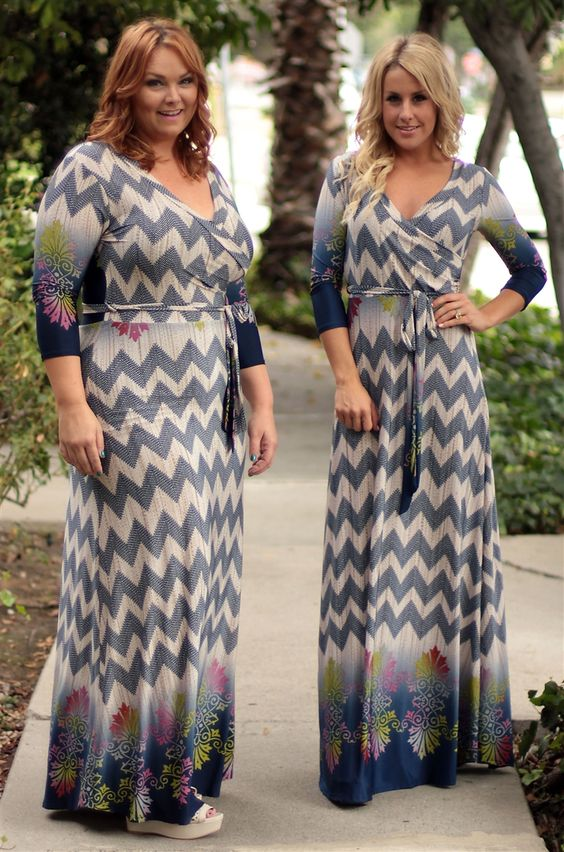
\includegraphics{dress_difference} 
\caption{The same dress on two different women with different shaped bodies}\label{fig: 2}
\end{figure}

	Along with the problem of clothing objects being deformable and worn on an articulated body, we also have to consider the other contextual aspects of an image. As intelligent humans, we can normally determine if a dress in an image is the same as another dress in another image, regardless of what other objects are in the background. When it comes to digital recognition, though, an image containing an explicit clothing item could be convoluted with other objects or people in the same image, or could have an explicit, plain background which takes over the image.

A method that is able to recognize and classify these objects must account for these degrees of freedom that come with the task. For instance, if we have the same object in multiple images with a white background, a computer may then recognize the background as being the defining feature of the image. When introduced to another image of the same object with a similarly noisy background, a computer may then think this is a different object altogether, because of the dramatic difference in backgrounds between this photo and the previous one(s). 
	
 \section{PUT A PICTURE OF A  VERY CONVOLUTED IMAGE HERE }

	The angle that a photo was taken and the location of a particular item in the image are also important considerations. All known images of an object could be front-facing, and if a side view of this object is introduced, a computer will have nothing to compare with this side view. In this event, the computer will not be able to correctly classify or recognize the object, since it has no previous knowledge of its side view. 

When worn, clothing items like shoes and hats are almost always near the bottom and top of an image, respectively (for obvious reasons). If a computer has only seen images of shoes in which they are located near the bottom edge of an image, the computer may think that this location is a common, fundamental characteristic of shoes themselves! This must be considered when choosing images for a computer to classify or match. A shoe, of course, can be anywhere in an image, and recognizing this when choosing images lets the focus be on features of the shoes themselves, rather than the object location. 
	
	Even if articulation, deformability, angle, and rotation have all been accounted for when attempting to classify and recognize objects, colour and illumination must also be added to this long list of considerations. Depending on the lighting conditions and the camera itself, the same red shirt may look pink in one image and orange in another (in fact, there was a viral internet sensation over a ?blue and black or white and gold? dress, a few years ago, due to this very perceptual issue). An image must be recognizable under different lighting conditions and in light of minor variations in the object's colour. 

Yet, what if an image of this shirt is in greyscale? This is an important question. If the goal is to recognize a red shirt in a given image, greyscale images cannot be considered. If they are considered, they must be accepted as either grey or colourless, even if the shirt in the image is actually red. In this case, the greyscale image is irrelevant. If the goal is to recognize a plain-coloured shirt, colour becomes unimportant, and a greyscale image can be as relevant as an RGB image.
	
 \section{PUT A PICTURE OF A SHIRT IN COMPLETELY DIFFERENT LIGHTING}
	
	When it comes to recognizing clothing items in images, it is naturally almost impossible to account for every possible variant from image to image. However, if we keep all the of degrees in freedom in mind when attempting to classify or match images, we can avoid many of the problems that come with such variations. 

Where do we start in terms of finding similarities in different images? One approach, and a good approach, is to find and identify specific features of an object which are common to almost every image of the object. Viola and Jones did this in 2004, with Real-Time Robust Face Detection. They classified faces in images, based on the computed values of simple features specific to the faces.\cite{viola2004robust}. They used simple rectangles (figure of Viola and Jones rectangles) to locate areas of brightness in a photo. If these specific areas of brightness are present, then the image contains a face. 

For our purposes, Viola and Jones' specific facial recognition, by design, only works with images of faces. Naturally, though, one would imagine that a similar process to this facial recognition could be used in attempting to recognize other objects in images, like clothing. In theory, we should be able to find prominent features that belong to any given type of clothing item, and use this feature to consistently classify the image.

%THIS IS A PARAGRAPH THAT HAS TO BE TAKEN APART	
	
	Multiple filters applied to the same image will give us multiple feature maps which can show us whether a specific feature is prominent in an image.\cite{aurelienMachineLearning}. If every image of a certain class in a training set is found to have a specific feature, a machine learning algorithm can use this feature to predict whether or not a given image belongs to this class.

For example, a filter that identifies horizontal lines in an image might be a good predictor for whether a pair of pants are present in an image, given that pants are straight and long. If this feature is found to be a good image predictor by a machine learning algorithm, and such horizontal lines are prominent in a new image, this image will be classified with pants. 
	
%ENDS HERE
		
	 As stated above, in images, we count on an item to have one or more identifying features, like a human face. One of the ways that we can find the parts in an image that are likely to be important, and make them more prominent, is by applying a filter to the image. 

A common example of a filter is the use of a neighbourhood operator, or local operator on pixels in an image. A neighbourhood operator uses an area of pixels around a specific pixel in an image to compute an output value for that pixel. When applied to all pixels across the image, the operator "filters" the image. A neighbourhood operator takes a weighted sum of all pixels in a neighbourhood. It is also known as a correlation, where h(k, l) are labelled the filter coefficients. 

A variant on this operator is the convolutional operator which is both commutative and associative. The convolutional operator is a reversal in f of the sign of the offsets g = f * h where h is now an impulse response function.\cite{szeliski2010computer}. 

\[g(i,j) = \sum_{k,l} f(k, l)h(i + k, j + l)\]
%That's a convolutional operator
	
	Filters can alter an image in dramatic ways. They can be used for edge detection, to blur photos, to adjust colour, or to sharpen images.\cite{szeliski2010computer}. Filters can play a crucial part in detecting any object in an image, as it makes it easier for a computer to recognize certain features in an image, but to manually find which features are important and which filters or convolution kernels work for each object is not always a feasible task. Filters are helpful in discovering features in an image and making them more prominent, but when dealing with 1000 or more images, how do we know which filters to use and what features are important? Machine Learning can help us "learn" things about these images, like which filters and convolution kernels work best, without having to manually go through the whole process. 

Simply put, Machine learning is programming a computer to learn something based on the data itself. People use machine learning to analyze and monitor data much more efficiently than executing it manually. It recognizes patterns, and can be used to learn what people are buying, which emails in your inbox are spam, and in this case, if a pair of jeans is in an image, and indeed which pair of jeans it is. \cite{aurelienMachineLearning}. 

Using machine learning algorithms, we can program a computer to learn about almost anything as long as we provide it with enough data, and the right data. For instance, if we want a computer to use machine learning to "learn" if a pair of shoes are present in an image, we have to make sure that we provide it with many images of many different kinds and brands of shoes, in different positions and orientations. These images are called our training set.\cite{aurelienMachineLearning}. The images in the training set are input into a machine learning algorithm. The algorithm then goes through the entire set of images and looks for similar features among all or most of the images. 
	
	The first step in this process of matching objects in images is to recognize (or correctly classify) a clothing item in an image. A machine learning algorithm needs to learn the way in which it will get the best results with the information available. This information is how a machine learning algorithm will be trained, hence the name "training set". After being trained, an algorithm should be able to predict the class of an object in an image. 

In other words, the predicted class, or label of a photo of a dress, should be one that refers to a dress. In this case, supervised learning will be used. With supervised learning, the algorithm already knows the class, or label, that each specific data element in the training set belongs to, and makes use of this for training purposes. If an algorithm predicts that a data element belongs to the wrong class while training, supervised learning lets the algorithm run again with the same data to attempt to correct its' previous mistakes\cite{aurelienMachineLearning}. Thus, a machine learning algorithm learns by making predictions on the same training set continuously until it can accurately predict the classes of all or most data elements in the training set. 
	
	How can supervised learning help in predicting which clothing item is in an image? Since we do not have to get everything right the first time with supervised learning, we can use a method that makes mistakes each time (or each epoch) that it iterates through our dataset. 

Neural networks are an effective way to do this. Like most machine learning algorithms or in this case deep learning algorithms, neural networks take one data element as input, and outputs a probability that this element belongs to each class in a list of classes. What is unique about neural networks is that they learn in a similar the way as a human brain. 

Neural networks are made up of a series of layers, and each layer is made up of one of one or more neurons, like the neurons in a human brain. Every neural network has an input layer made up of input neurons, an output layer made up of output neurons, and 1 or more hidden layers composed of hidden neurons. 

For the purpose of explanation, an example will be given, with only one hidden layer. In the figure below, there is three input neurons, or signals: x1, x2, and x3. Each neuron in the input layer is connected to each neuron in first hidden layer. A neuron in the first hidden layer is fed the input from all input neurons, and each one of these inputs has a weight applied to it by multiplication. In this hidden neuron, all inputs are multiplied by their respective weights, and added together. This sum is then given to an activation function. The output of this activation function is the output value of this hidden neuron. This is done for each neuron in the first hidden layer. If there are more hidden layers, the output of the previous hidden layer's neurons are fed into the neurons in these layers as input. This continues until the output layer is reached, where each output neuron represents a specific class and calculates the probability that the input belongs to this class.\cite{KubatMachineLearn}
	
 	A Neural network has input neurons and output neurons, but how does it learn, and how is it supervised? Back-propagation takes the same input through a network to correct any mistakes made in previous predictions (probabilities of classification). This is where the training set comes in. 

During each Epoch of a training session, each element in the training set is forward-propagated through the neural network. Since we know the correct classification of all elements in our training set, after each epoch we can compute the error in the classification. This can be done using the weights. Since all neurons contribute independently to the classification of the input, each input or hidden neuron in a particular layer has a different weight to carry it to each neuron in the next layer. All weights should be updated by adjusting for the error in the previous epoch. A neural network should improve at predicting the actual class of its input after every training epoch. The error of an entire output layer can be calculated using accuracy, precision, or recall. Each one of these calculations can tell us how close the network was to making a correct prediction. 

Once a neural network is properly trained, the same weights can be used over and over to make predictions. This process of using error to back-progate through a network using weights can help a network to learn almost anything.\cite{KubatMachineLearn} 
	
	Since neural networks can learn almost anything, one would expect that they could learn which objects are in an image, or if an image contains a particular clothing item. They can, but with a bit of an adjustment. A specific type of deep neural network is used for image classification called a convolutional neural network. 

Convolutional neural networks have a similar flow to other neural networks. The input is all pixel values in an image and the output is again the probability that the input belongs to a certain class. In this case the output will be the probability that the input image contains a certain object. 
	
	A variation on filtering is a convolution.
\bibstyle{acm}
\bibdata{References}
\end{document}

